\section{Implementation}
\label{section-implementation}

In this section we describe our implementation of SpartanRPC. We have created a program we call
\emph{Sprocket} \cite{sprocket} that accepts a SpartanRPC enabled nesC program and outputs an
ordinary nesC program.

We focus here on describing the highlights of the implementation. In Sprocket, a duty posting is
converted into a remote message send, containing an \emph{identifier} associated with the posted
duty so the receiver may dispatch the intended functionality. The RPC service provider runs a
\emph{skeleton} of any remotable interface, that receives these messages, interprets
identifiers, and dispatches functionality appropriately. Dynamic wirings in RPC client programs
are converted to statically wired \emph{stubs}. When a duty posting is converted into a message
send by Sprocket, the component IDs in the dynamic wiring endpoints are integrated into the
message. To support security features, duty messages may also contain a MAC computed with an AES
key associated with a particular capability; authentication of this MAC underlies SpartanRPC
authorization.

\subsection{Identifiers}

A SpartanRPC identifier is a 4-tuple $(N, C, I, D)$. Here, $N$ is the TinyOS ID of the node on
which the duty is implemented; we assume that these are network-level unique. $C$ is a component
ID assigned to each component that provides a remotable interface; component IDs are node-level
unique. $I$ is an interface ID, required since a component may provide more than one remotable
interface, even multiple instances of the same interface. Finally, $D$ is a duty ID, which must
be interface-level unique.

In the current version of Sprocket, IDs are assigned statically by an arbitrary (automated
and/or social) process, and we assume that Sprocket configuration files that define the
association between IDs and the entities to which they refer are known to all interacting
actors. More sophisticated techniques for defining and communicating RPC interface definitions
between actors is an interesting topic for future work.


\subsection{Data Packet Format}
\label{section-packet-format}

SpartanRPC packets contain a header with addressing information and marshalled duty arguments.
The total size of a SpartanRPC data packet is limited to 16 bytes in the current version of
Sprocket. (or 20 bytes when authentication is used). Fig.~\ref{fig:packet} shows the packet
format.

\begin{figure}[!t]
  \centering
  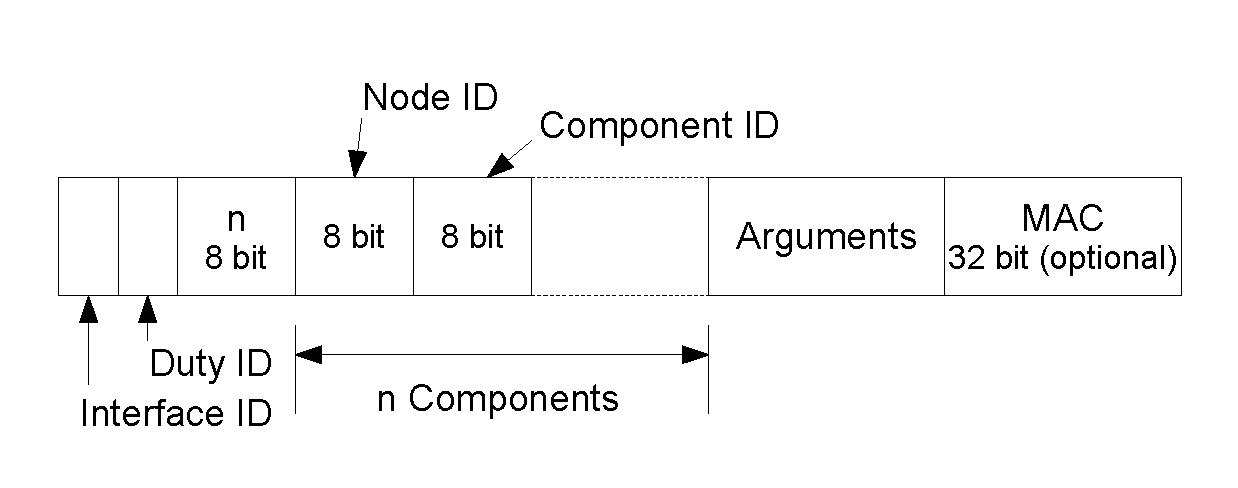
\includegraphics[scale=0.43]{packet}
  \caption{SpartanRPC data packet format.}
  \label{fig:packet}
\end{figure}

The SpartanRPC packet header can introduce significant overhead in some cases. In the current
version of Sprocket, $I$ and $D$ are packed as two four bit fields in a single byte. Each
intended destination is identified by a byte for $N$ and a byte for $C$. Finally an additional
byte is used to encode the header's size. This yields a total overhead of $2 + 2n$ bytes where
$n$ is the number of components intended to receive the packet. A special node ID of \code{0xFF}
is used to represent a SpartanRPC level broadcast. Thus in the special (and common) case where
all neighbor nodes are to process the remote call the overhead is exactly four bytes, leaving 12
bytes for duty parameters. If a parameterless duty is called, the maximum fan out supported by
our implementation is seven.

The limited field sizes used in the header put static restrictions on the system. Only 16 remote
interfaces per component can be used with at most 16 duties per interface. In addition, the
current version of Sprocket limits the network to at most 255 nodes with 256 remotely accessible
components per node.

\subsection{Skeleton Generation}

For each remote interface provided, Sprocket converts the duties in the component providing that
interface into nesC commands. Sprocket also generates a skeleton component for every remote
interface implementation. These skeletons are connected to the active message components in the
TinyOS library. Each time a duty message is received the skeleton checks the packet for
applicability. If the packet is not intended for the $(N, C, I)$ triple supported by the
skeleton or if $D$ is out of bounds for the interface, the packet is ignored. In the interest of
minimizing radio traffic, no error indication is returned.

If the packet is applicable, the skeleton unmarshalls the message, stores the duty arguments in
skeleton-local variables, and posts a task that implements the duty. For each duty in the
provided interface, Sprocket generates a trivial task in the skeleton that simply calls the
converted duty. For example:
\begin{Verbatim}
// 'value' written when packet unmarshalled.
uint8_t value;
task void setLeds()
    { call Blink.setLeds(value); }
\end{Verbatim}
\vspace{0.3em}

Thus the task-like semantics of duties are ultimately implemented in terms of ordinary nesC
tasks.

\subsection{Stub Generation}

On the RPC client side, Sprocket converts each duty posting into a command in a stub component
generated by Sprocket. That command first calls the \code{elements} command in the component
manager to obtain the list of target components. It then prepares a SpartanRPC data packet by
marshalling the duty arguments. Finally it broadcasts the packet to all neighboring nodes using
the TinyOS active message library. Recipients discern packets intended for them via packet
identifiers as described above.

Sprocket converts dynamic wires into static wiring that connects the posting component to the
generated stub. The stub is connected to the component manager associated with the dynamic
wiring. For example, a dynamic wire such as:
\begin{Verbatim}
ClientC.LEDControl ->
    [RemoteSelectorC].LEDControl;
\end{Verbatim}
is converted converted into the configuration as follows:
\begin{Verbatim}
components Spkt__1;
ClientC.LEDControl -> Spkt__1;
Spkt__1.ComponentManager -> RemoteSelectorC;
Spkt__1.Packet    -> AMSenderC;
Spkt__1.AMPacket  -> AMSenderC;
Spkt__1.AMControl -> ActiveMessageC;
Spkt__1.AMSend    -> AMSenderC;
\end{Verbatim}

The \code{Spkt\_\_1} component is the Sprocket generated stub.

\subsection{Security}

When capability-based security is used, Sprocket consults a configuration file that maps
capabilities to keys. To activate a capability over a dynamic wire, the Sprocket generated stub
computes a MAC that covers the SpartanRPC header and marshalled duty arguments. In the current
implementation this MAC is computed using the AES encryption algorithm in CBC mode with an
initialization vector of zero. Because SpartanRPC packets are currently limited to 16 bytes,
only a single AES encryption is necessary to compute the MAC. The first four bytes of the
resulting cipher text is used as the MAC value. While a MAC of only 32 bits would not normally
be considered secure, wireless sensor networks generate data so slowly that attacking even such
a short MAC is not considered feasible \cite{karlog-tinysec-2004,luk-minisec-2007}. Our MAC
computation is simplistic, but we feel it is adequate to demonstrate a proof of concept.

For components providing a secure remote interface, the generated skeleton incorporates a MAC
authentication procedure under the required key as declared in the component specification. The
usual checks of interface ID and component ID are done first so as to avoid a costly MAC
computation in the case where the received packet is not actually intended for the skeleton.
Only when the other applicability checks succeed is the MAC checked. The duty invocation is
ignored if the MAC check fails.
